% link naar figuurtje over Tor
\section{Tor}
	\label{scc:tor}
	Tor, the second generation onion router, is a privacy-enhancing overlay network. Onion routing was first described by Chaum in his paper "Untraceable electronic mail, return addresses, and digital pseudonyms" \cite{chaum1981untraceable}. Tor is the most widely used and secure implementation of onion routing. It was first implemented in 1996 by the U.S. Navy Research Laboratory as a means to protect government and military communications from digital and physical attacks \cite{goldschlag1996hiding}.
	
	Tor uses the principle of onion routing to ensure secure communication between parties. Network traffic is encrypted and forwarded over a circuit of nodes. Each node in this circuit only knows the previous and next node. The communicating parties stay hidden when this circuit of independent nodes is sufficiently long.
	
	\begin{figure*}[!t]
		\centering
		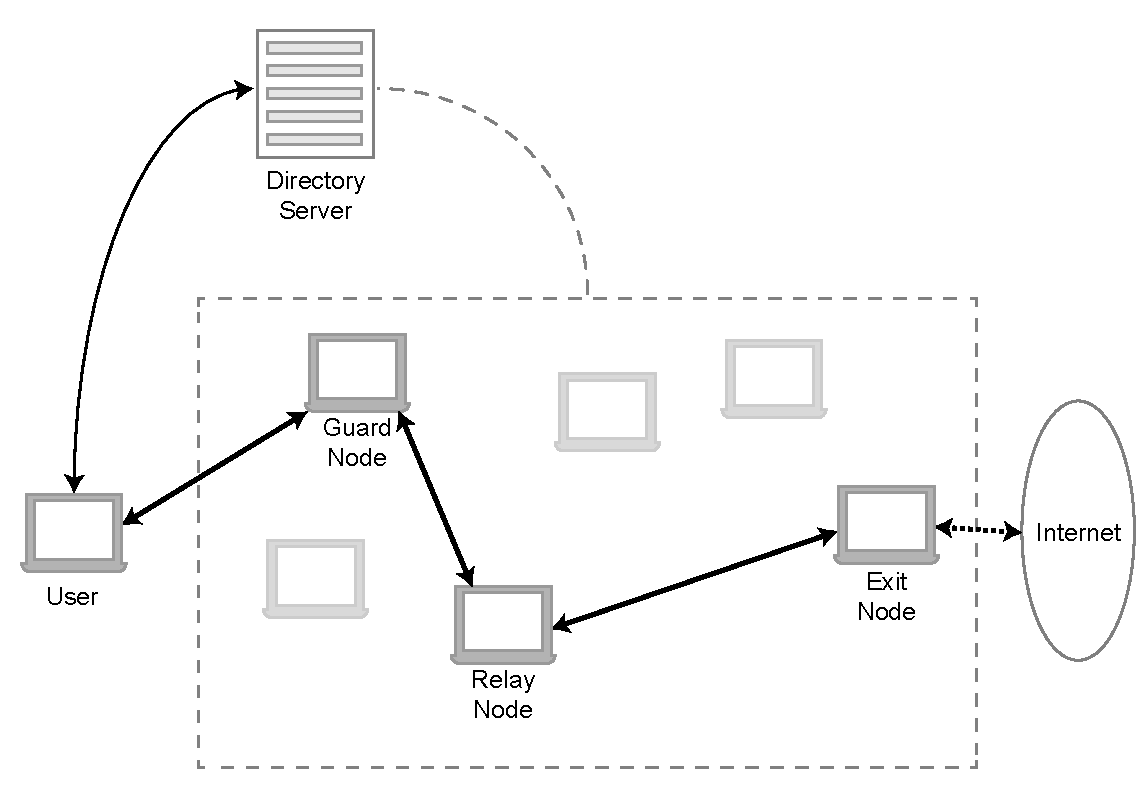
\includegraphics[width=0.8\textwidth]{prior-work/tor.pdf}
		\caption{The components of the Tor network. After downloading the node list from the Directory Server, the user creates a circuit through a guard node, a relay node and an exit node. This circuit is used to communicate (anonymously) with the Internet.}
		\label{fig:tor_layout}
	\end{figure*}
	
	There are several drawbacks to the current implementation of Tor, see Figure \ref{fig:tor_layout}. Centralized components, such as the directory server, act as a bottleneck and limit the number of possible users \cite{jagerman2014fifteen}. Since anonymity in a network such as Tor is directly linked to the number of active users this is an alarming situation.
